\section{The TSTL Harness Language}
\label{sec:lang}

The TSTL compiler takes as input a harness template file, and produces
as output a Python class file that implements an interface other tools
can use to perform testing on the SUT via an SUT-independent interface.

The harness in Figure \ref{fig:MakeFeatureLayer} shows many of the
basic features of TSTL.  The basic structure of a TSTL harness
consists of three parts, usually written in order.  First, harness
code prefixed by an {\tt @} or enclosed in {\tt <@ @>} is treated as
raw Python code, and essentially not interpreted by the TSTL
compiler.  This code is reproduced almost literally in the output
file\footnote{TSTL does have to scan {\tt import}s to re-load modules, and also pre-processes function
  definitions to support
pre- and post-conditions.}.  Second, there is a preamble that almost
always defines a set of \emph{value pools} for use in testing, but
also may include information on logging, correctness properties,
source code locations for code coverage analysis, and other basic
information that applies to the entire harness.  Finally, the bulk of
a TSTL harness (and the only non-optional element) is a set of
\emph{action definitions}.  Actions are the possible steps to be taken in
testing, and define the set of possible tests.

The original version of TSTL \cite{NFM15} required cumbersome use of Python
functions to implement many simple operations, including guards.  Current TSTL extends
the language to make it possible to define very complex test spaces
using only pools and actions, with helper functions only required for
the usual reasons of abstraction and readability.

\subsection{The Essentials of Pools and Actions}

In TSTL, tests usually consist of assignments to value pools and uses of the
values in those pools.  In order to make the core ideas clear,
consider part of Figure \ref{fig:MakeFeatureLayer}, defining how to
generate values used in SQL where clauses.  The following, by itself,
is a valid TSTL harness (albeit one that cannot discover any
interesting faults):

{\scriptsize
\begin{code}
pools:
  <val> 2 CONST
\vspace{0.05in}
actions:
\vspace{0.05in}
<val> := <1..10>
<val> = <val> + 1
\end{code}
}

There is only one pool, named {\tt val} (optionally labeled as {\tt CONST} to
indicate that its value does not change unless it appears on the left
hand side of an assignment).  The pool has room to store
two values.  The state of the SUT is defined by the state of all
pools.  Initially, all pools are set to a special value ({\tt None}) indicating the
pool has not been initialized.  Pools can be thought of as 
normal Python variables, for the most part, so we can think of the
{\tt val} pools as variables {\tt val0} and {\tt val1}.

Actions that include the {\tt :=} form of assignment (a TSTL, not
Python, operation) initialize pool values.  When {\tt <val>} appears
in an action, that represents all possible pool locations with that
name:  for our simple example, either {\tt val0} or {\tt val1}.  An
integer range is represented by {\tt <i..j>}, and TSTL expands such
ranges to produce an action with each possible choice. The
first line in the actions section of this harness translates to 20
different possible actions:

\begin{figure}
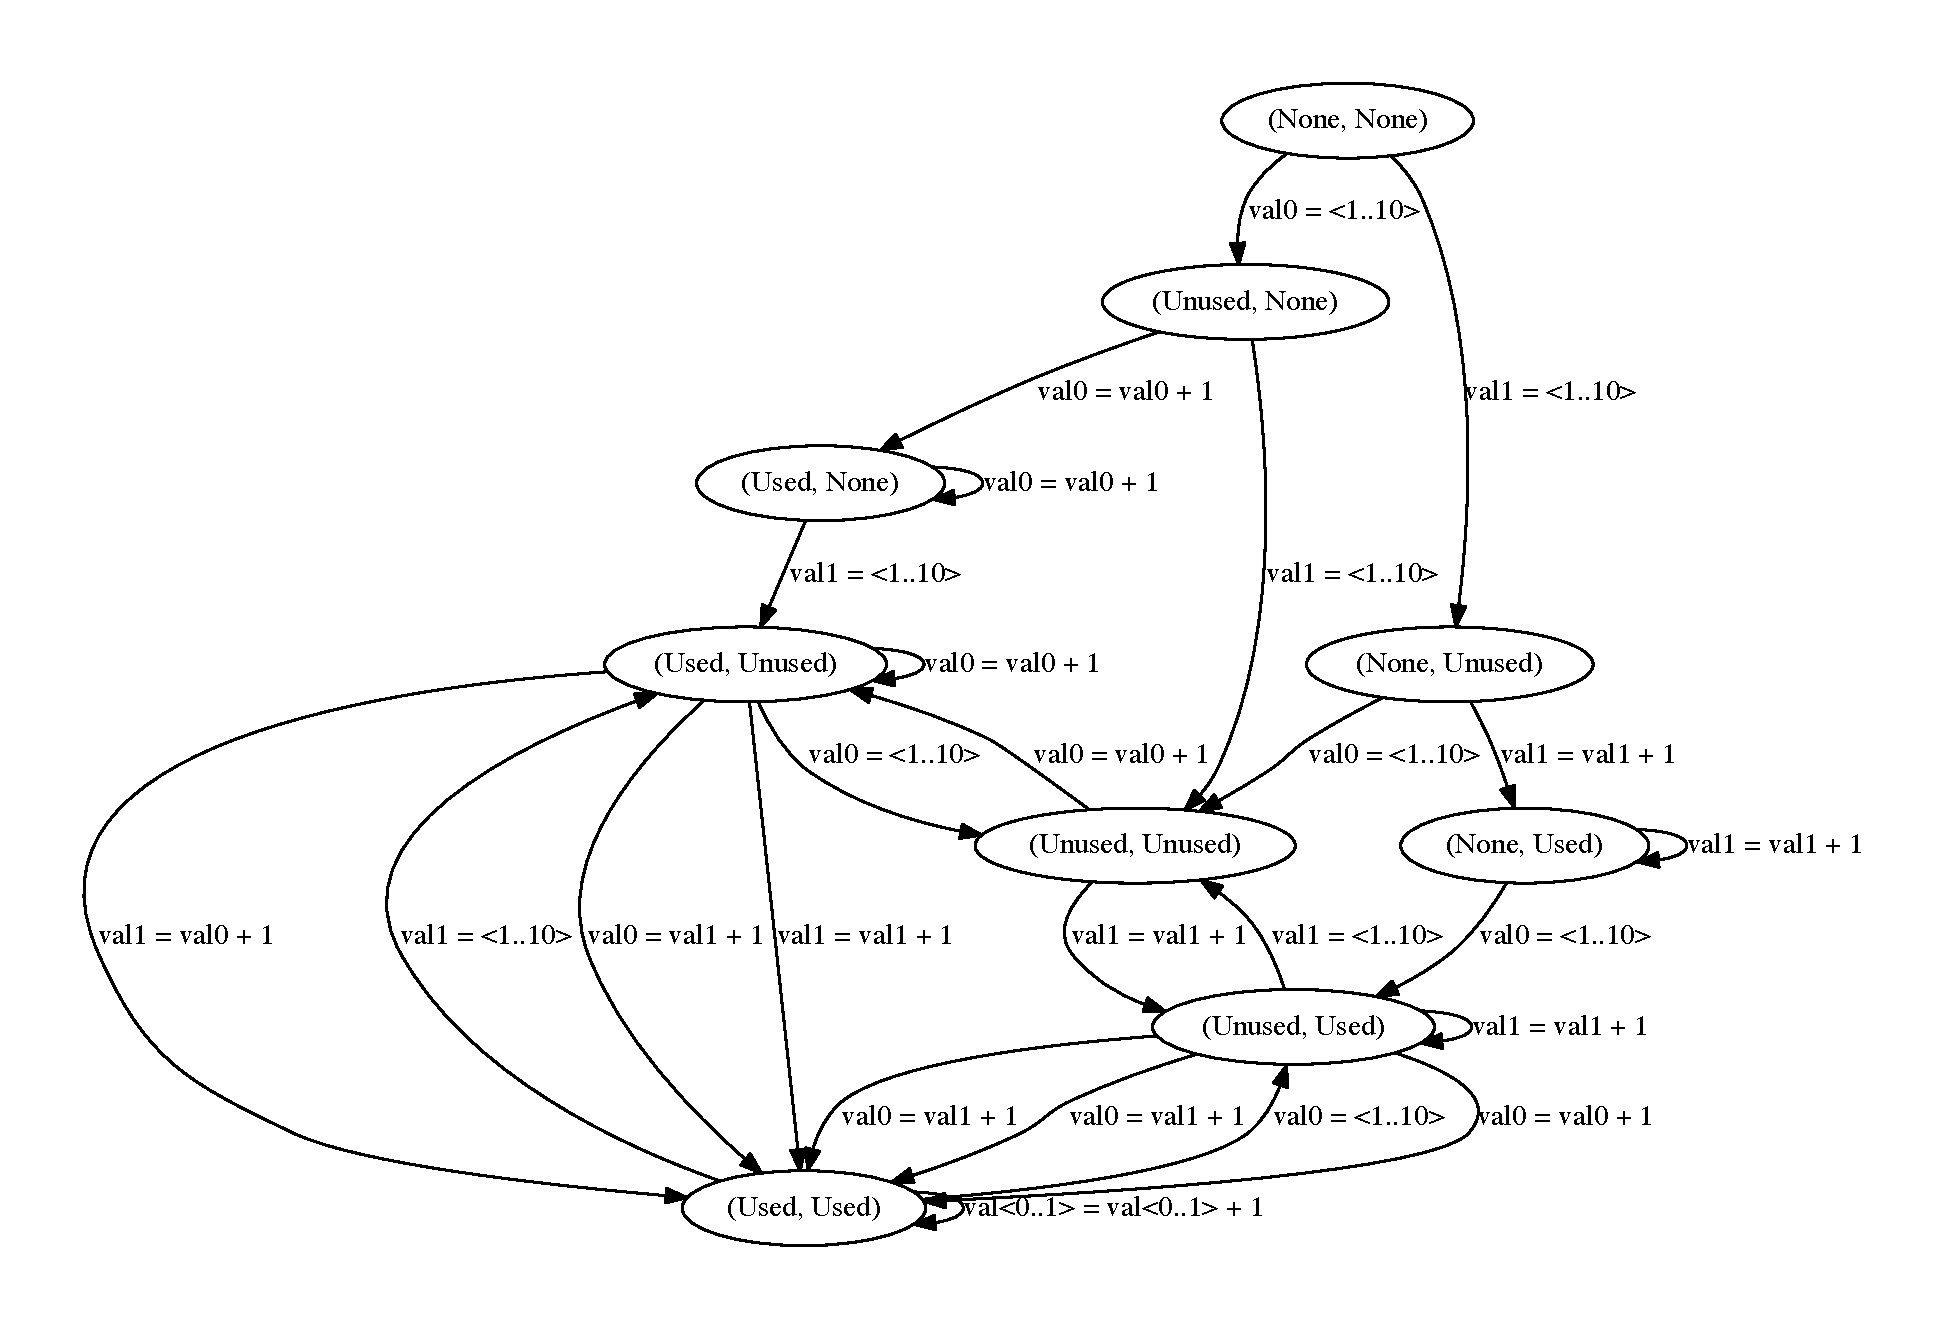
\includegraphics[width=\columnwidth]{states}
\caption{Constraints on actions in a test, based on pool states}
\label{fig:poolacts}
\end{figure}

{\scriptsize
\begin{code}
val0 = 1
val0 = 2 ...
val0 = 10
val1 = 1 ...
val1 = 10
\end{code}
}

From the initial state of the system, only these 20 actions are
\emph{enabled}.  \emph{Enabled} actions are those that can be executed in the
current state; the complete set of actions defined by a TSTL harness is always
finite, and the enabled set is always a subset of that finite set.  The first concept that is essential to understanding
TSTL semantics is that at any state of the
system, the only actions that are enabled are those that do not
\emph{use} any non-initialized pool values.  Any appearance of a pool
value is considered a \emph{use}, with the single exception of the left-hand-side of a
{\tt :=} initialization (not normal assignment)\footnote{The definition of
use is the only distinction between {\tt :=} and normal Python
assignment; {\tt :=} is implemented as Python assignment, and appears
as such when test cases are printed.}.  The second concept is that a
value that has been initialized
cannot be initialized (appear on the lhs of {\tt :=}) until after at
least one action
that uses it has been executed.  Figure \ref{fig:poolacts} shows the
consequences of these rules for the simple value assignment harness
above.  The nodes in the graph are labeled with {\tt state(val0),
  state(val1)}, where state is
either {\tt None} (uninitialized), {\tt Unused} (initialized
but never used) or {\tt Used} (initialized and used at least once).
Starting from the initial state {\tt (None, None)}, a valid test is any path
through the graph. 

Tests that can be produced by this harness include, therefore,
sequences like  {\tt val0 = 3; val0 = val0 + 1; val1 = 4; val1 = val0
  + 2} and {\tt val1 = 10; val0 = 6; val0 = val1 + 1; val0 = 2; val1 =
  15}.  However, {\tt val0 = val0 + 1; val0 = 2} and
{\tt val0 = 1; val1 = 1; val1 = 4} are not valid tests, because they
either use an uninitialized pool value, or re-initialize an unused
pool (a clearly useless action sequence).

\subsection{Other Core Language Features}

The example TSTL harness in Figure \ref{fig:MakeFeatureLayer} shows a
few other important core elements of TSTL.  First, choice templates
are not limited to integer ranges, but can include arbitrary items in
a list, e.g, {\tt <fc> := <["d1.shp", "d2.shp", "d3.shp"]>}.
Normally, when an action raises an uncaught exception, this is
considered a test failure.  Prefixing an action with a set of
exception names in curly braces (e.g., {\tt \{IOError\}}) indicates
that some exceptions are expected, and do not indicate a failure.
More critically, actions can be prefixed by arbitrary guards, using
the syntax {\tt guard -> action}.  The simple ArcPy harness chooses
field names for SQL by first extracting a list of all fields in some
feature class.  It then allows a field name to be chosen by taking the
name of the first field in the list.  However, since the harness also
allows the list of fields to be stepped through by discarding the
initial element, the name extraction has to be guarded to ensure that
tests won't try to extract names from an empty field list:  {\tt
  len(<fieldlist,1>) >= 1 -> <fieldname> := <fieldlist> [0].name}.
The {\tt <fieldlist,1>} construct, which can also be used outside of a
guard, indicates that this pool value should not be produced using
normal template expansion (instantiated as both {\tt fieldname0} and
{\tt fieldname1}) but rather than it should copy the comma indexed
appearance of that pool in each expansion (indexing starts from 1).  This makes sure the guard
is over the same pool value that is used in the action.

TSTL also supports post-conditions on actions, in the form {\tt action
  => post-condition}, where an assertion is checked after certain
actions are performed.  For example, because some known ArcPy bugs
involve addition of incorrect characters to field names in a database,
we could add code to check that field names in feature classes never
change from their initial values.  We can make sure that a library
call to add a field to a feature class adds it to a database of all
field names collected at the start of testing, and check the set of
values returned for each feature class at the beginning of each test,
and store these in a dictionary.  This example code shows two more
features of TSTL: TSTL supports {\tt init:} code in the preamble,
which is called before each test starts.  Ending a line in a backslash
indicates the action continues on the next line of the file.

{\scriptsize
\begin{code}
init: <fieldnames> = getAllFieldNames(getFeatureClasses())

\{ExecuteError\} not (<fc,1> in <hascursor>) -> \\
   AddField\_management(<fc>,<fieldname>,<fieldtype>); \\
   <fieldnames> [<fc,1>].add([<fieldname,1>])

\{IOError\} <fieldlist> := ListFields(<fc>) \\
  => sorted(<fieldlist,1>) == sorted(list(<fieldnames> [<fc,1>]))
\end{code}
}

Note the additional guard on adding fields --- we have discovered that
adding a field to a feature class that has any database cursors active
tends to crash ArcPy.  For more complicated post-conditions, the construct {\tt
  pre<(expr)>} allows access to values of expressions from before the
action was executed, as a further convenience for expressing properties.

When a correctness property is more general than a post-condition on a
single action, it can also be included in the preamble, to be checked
after every action.  Our field name property could therefore also be
stated as {\tt property: sorted(ListFields(<fc>)) ==
  sorted(list(<fieldnames> [<fc,1>]}.  Rather than checking only the
feature class whose fields have been extracted, this will expand to a
check for all feature classes.  The advantage is that the property will
catch problems even if we never construct a {\tt fieldlist}; the
disadvantage is that testing slows to check all field names for all
feature classes, after every action.

Another useful feature of TSTL is the ability to create
\emph{reference} pools, where every action on pool values is mirrored
by an action on a reference version of that pool.  This makes it
possible to perform differential testing \cite{Differential} on a
per-pool basis, rather than at the whole-system level, allowing
complex partial specifications.  For example, in ArcPy we may want to
ensure that operations are deterministic: no GIS operations produce
different results, given the same underlying starting feature class
data.  Assuming in raw Python in the preamble we have defined {\tt
  identityFunction} as an identity function and {\tt copyFCName} as a
function that takes a feature class name and transforms it into a
generated name for a reference copy of the feature class, the
following mirrors all actions on feature classes on a reference copy,
and checks that the feature class and its reference always have the
same fields.

{\scriptsize
\begin{code}
pools:
  <basefc> 2 CONST
  <fc> 2 CONST REF

<basefc> := <[``d1.shp'', ``d2.shp'', ``d3.shp'']>; \\
  CopyFeatures\_management(<basefc,1>,copyFCName(<basefc,1>)
<fc> := identityFunction(<basefc>)
\{IOError\} <fieldlist> := ListFields(<fc>)

references:
  identityFunction ==> copyFCName

compares:
  ListFields
\end{code}
}

When instantiating the action templates, TSTL always produces a copy
of every action containing any reference pool values.  First, the pool
values are replaced with their reference copies; second, all the
syntactic transformations (which can include arbitrary Python regular
expressions) in the {\tt references} declaration are applied.
Finally, if any string matches a regular expression in a {\tt
  compares} declaration, the return values or assigned values in the
action are compared with those for the reference version.  In the
ArcPy case, if our {\tt copyFCName} is correctly defined, we can even
check that behavior is equivalent for different underlying data file
format for feature classes.

\subsection{How to Build a TSTL Harness}

In the introduction, we noted that one problem with automatic
extraction of harnesses by tools is that in order to effectively test
complex systems, it is important to incrementally build testing
capability, understanding the effort as it increases in scope.  TSTL
naturally supports this methodology.  The ArcPy harness, though
complex, was developed by starting with a small number of ArcPy
functions, and determining their parameters.  These functions were
chosen because they were involved in unusual or problematic behavior
experienced by the authors of the paper.  Once
functions have been chosen, and their parameters are known,
developing a harness can often be a clean, iterative process:

\begin{enumerate}
\item Choose a new function (or set of related functions) to include
  in the harness.
\item Determine all parameters types.
\item If there is no pool that can produce these types, determine how
  to produce these types, and add pools and pool initialization actions for
  those pools.  This may require adding some additional
  functions (in which case, go to step 1 and start with those
  functions).
\item Add an action to call the function(s) being added.  If relevant,
  allow any expected exceptions, guards, and post-conditions to check.
\item Run testing, examine code coverage and failures to evaluate the
  added code, and repeat from step 1.
\end{enumerate}

These steps, combined with occasional refactoring or generalization of
parts of the harness, can effectively test even a large library, while
maintaining tester understanding and control.   In the ArcPy test
harness development, most of the effort was spent in this cycle, with
major exceptions being the implementation of a method allowing users
to provide their own GIS data as a basis for testing, and efforts to
improve the TSTL tool infrastructure to support testing a complex
application in a Windows environment.